\documentclass[aspectratio=169]{beamer}
%[handout]

\usetheme[progressbar=frametitle]{metropolis}
\usepackage{appendixnumberbeamer}

\usepackage[utf8]{inputenc}
\usepackage[T1]{fontenc}

\usepackage[brazil]{babel}
\usepackage[outputdir=..]{minted}
\usepackage{xcolor}
\usepackage{soul} % strikethrough
\usepackage{advdate}
\usepackage{graphicx}
\graphicspath{{figs/}}
\usepackage{graphbox}

\usepackage[ampersand]{easylist}

\usepackage{multirow}
\usepackage{multicol}
\usepackage{subcaption}

\usepackage{pgf,tikz}
\usetikzlibrary{shapes,arrows,positioning}
\usetikzlibrary{circuits.logic.US}
\usetikzlibrary{matrix,calc}

\usepackage{karnaugh-map}

\usepackage{pgfpages}
\setbeameroption{hide notes} % Only slides
% \setbeameroption{show only notes} % Only notes
% \setbeameroption{show notes on second screen=right} % Both

% \graphicspath{{../figs/}}

\definecolor{bgc}{rgb}{0.95,0.9,0.95}
\definecolor{links}{HTML}{2A7F7F}
\hypersetup{colorlinks,linkcolor=,urlcolor=links}

\newminted{verilog}{fontsize=\scriptsize, 
    linenos,
    numbersep=8pt,
    bgcolor=bgc,
    tabsize=4,
    framesep=3mm} 
    %frame=lines,

\newcommand{\verilog}[1]{\verilogf{#1}{\footnotesize}}

\newcommand{\verilogf}[2]{\inputminted[fontsize=#2, 
    linenos,
    tabsize=2,
    numbersep=4pt,
    bgcolor=bgc,
    framesep=3mm]{verilog}{../codes/#1.v}
}

\newminted{nasm}{fontsize=\scriptsize, 
		   linenos,
		   numbersep=8pt,
           bgcolor=bgc,
		   framesep=3mm} 

\usepackage{booktabs}
\usepackage[scale=2]{ccicons}

\usepackage{pgfplots}
\usepgfplotslibrary{dateplot}

\usepackage{hyperref}


\usepackage{xspace}
\newcommand{\themename}{\textbf{\textsc{metropolis}}\xspace}



\usepackage{pifont}% http://ctan.org/pkg/pifont
\newcommand{\cmark}{\ding{51}}%
\newcommand{\xmark}{\ding{55}}%

% \tiny	
% \scriptsize
% \footnotesize
% \small	
% \normalsize	
% \large	
% \Large	
% \LARGE	
% \huge	
% \Huge	



\newminted{python}{fontsize=\scriptsize, 
		   linenos,
		   breaklines,
		   numbersep=8pt,
           tabsize=2,
		   framesep=3mm} 
		   
\newminted{verilog}{fontsize=\scriptsize, 
		   linenos,
		   breaklines,
		   numbersep=8pt,
           tabsize=2,
		   framesep=3mm} 
		   




\definecolor{bgc}{rgb}{0.95,0.9,0.95}
\definecolor{links}{HTML}{2A7F7F}
\hypersetup{colorlinks,linkcolor=,urlcolor=links}


% \usepackage[style=apa]{biblatex}
% \addbibresource{mm.bib}


% \author{\large Prof. Ricardo Menotti (\href{mailto:menotti@ufscar.br}{menotti@ufscar.br})}

\newcommand{\newauthor}[2]{
  \parbox{0.50\textwidth}{
    \texorpdfstring
      {
        \centering
        \small #1 \newline
        {\scriptsize{\urlstyle{same}\href{mailto:#2}{#2}\urlstyle{tt}}}
      }
      {#1} \newline
  }
}

\author{
  \newauthor{Prof. Ricardo Menotti}{menotti@ufscar.br}
\and \newauthor{Prof. Luciano de Oliveira Neris}{lneris@ufscar.br}  
%\and \newauthor{Prof. Artino Quintino da Silva Filho}{artino@ufscar.br}
% \and \newauthor{Prof. Maurício Figueiredo}{mauricio@ufscar.br}
% \and \newauthor{Prof. Edilson Kato}{kato@ufscar.br}
% \and \newauthor{Prof. Roberto Inoue}{rsinoue@ufscar.br}
}

\date{Atualizado em: \today}

\institute{\large \textbf{Departamento de Computação} \\
Centro de Ciências Exatas e de Tecnologia \\
Universidade Federal de São Carlos}

\title{Lógica Digital (1001351)}

\titlegraphic{\hfill
\includegraphics[height=1.5cm]{LogoUfscar}}



\setbeameroption{hide notes} % Only slides
%\setbeameroption{show only notes} % Only notes
% \setbeameroption{show notes on second screen=right} % Both
% See: https://gist.github.com/andrejbauer/ac361549ac2186be0cdb

\subtitle{Síntese lógica} % 

\begin{document}

\begin{frame}
	\titlepage
\end{frame} 

% Uncomment if you want a summary slide
% \begin{frame}{Conteúdo}
% 	\tableofcontents
% \end{frame}

\section{Síntese Lógica}

\frame{     \centering
    \frametitle{\insertsection}
    \begin{columns}
        \begin{column}{0.40\textwidth}
            %\vspace{3cm}
            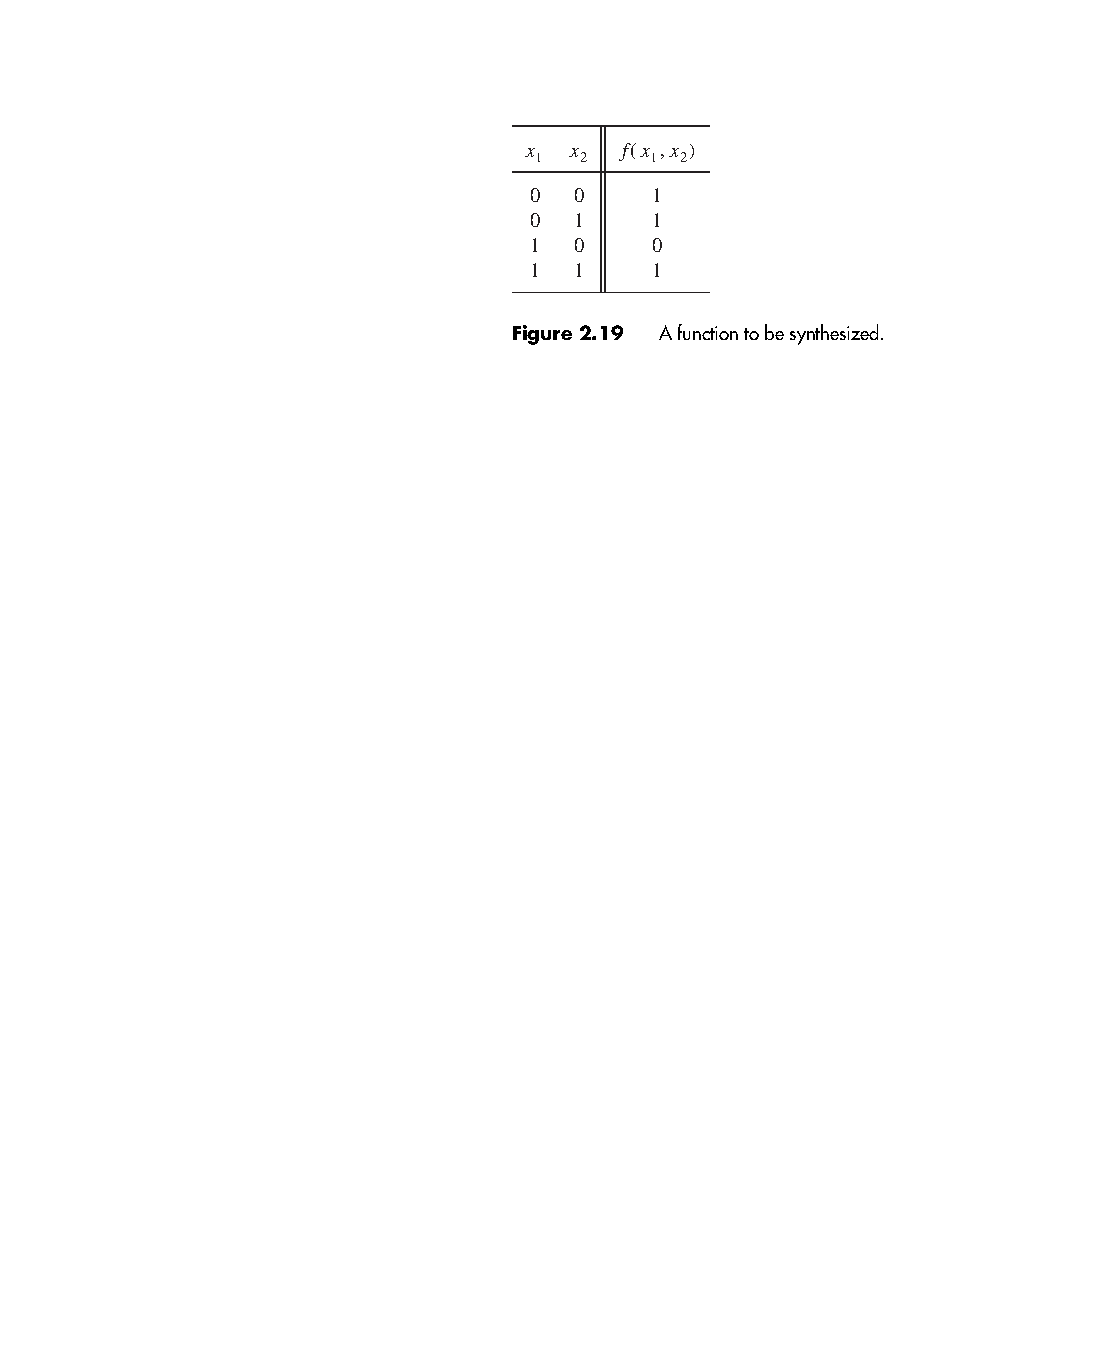
\includegraphics[width=1.5\textwidth]{VerilogFig2_19}
        \end{column}        
        \begin{column}{0.60\textwidth}
            $f(x_1,x_2)=x_1x_2+\overline{x}_1\overline{x}_2+\overline{x}_1x_2$
            $f(x_1,x_2)=x_1x_2+\overline{x}_1\overline{x}_2+\overline{x}_1x_2+\overline{x}_1x_2$
            $f(x_1,x_2)=x_1x_2+\overline{x}_1x_2+\overline{x}_1\overline{x}_2+\overline{x}_1x_2$
            $f(x_1,x_2)=(x_1+\overline{x}_1)x_2+\overline{x}_1(\overline{x}_2+x_2)$
            $f(x_1,x_2)=1.x_2+\overline{x}_1.1$
            $f(x_1,x_2)=x_2+\overline{x}_1$
        \end{column}
    \end{columns}
}

\frame{     \centering
    \frametitle{\insertsection}
    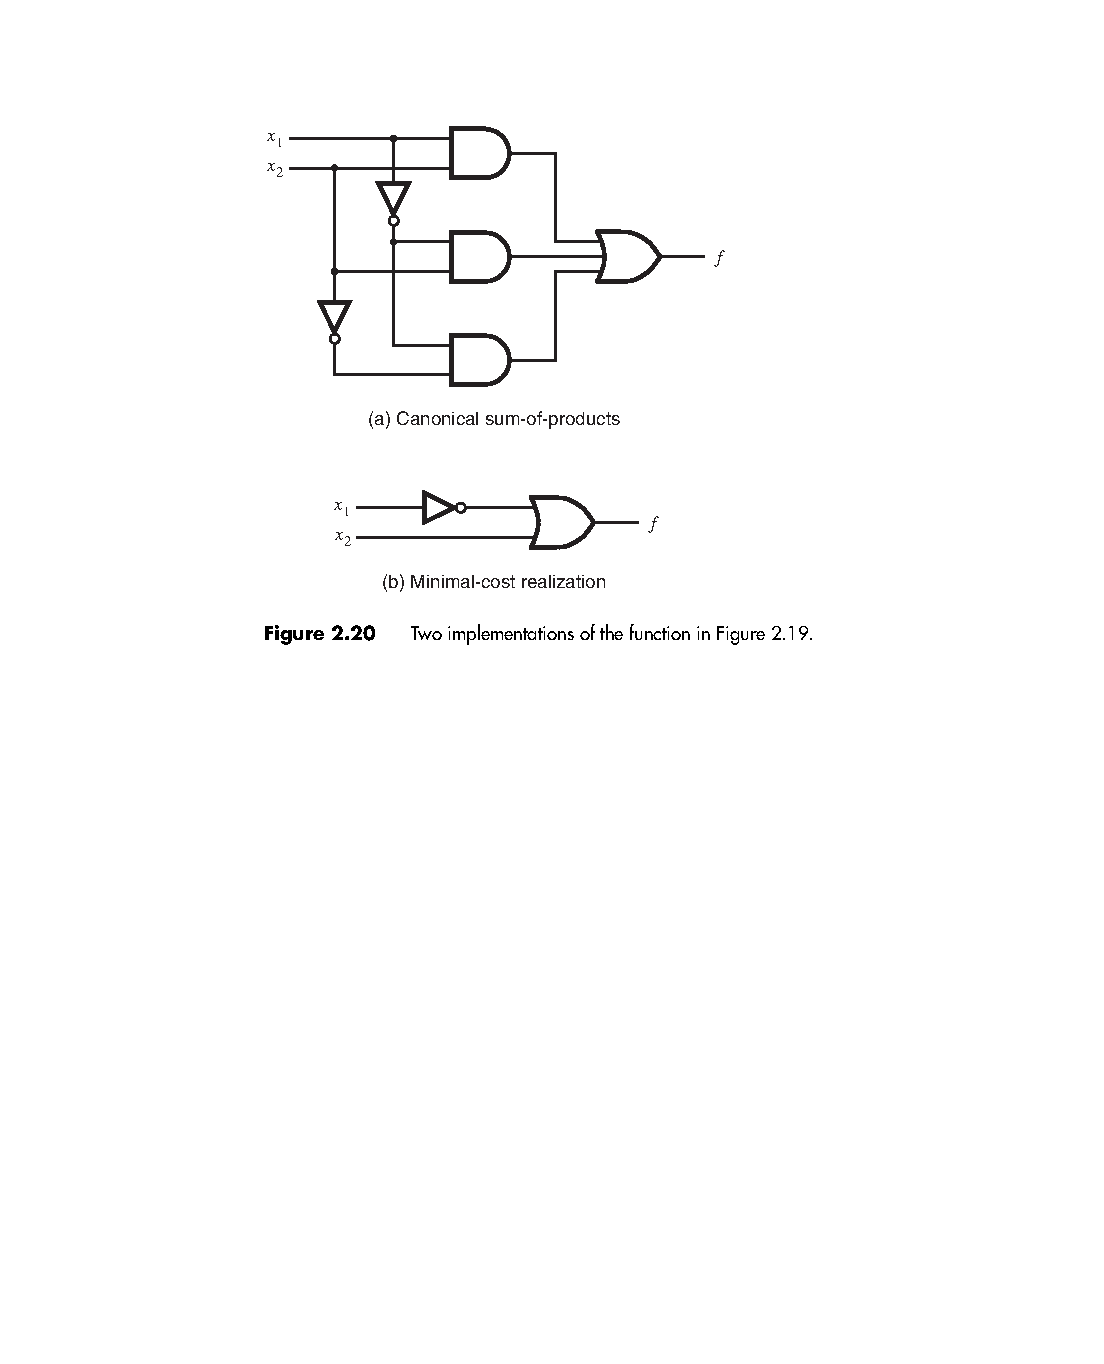
\includegraphics[scale=.8]{VerilogFig2_20}
}

\frame{     \centering
    \frametitle{\insertsection}
    \begin{columns}
        \begin{column}{0.45\textwidth}
            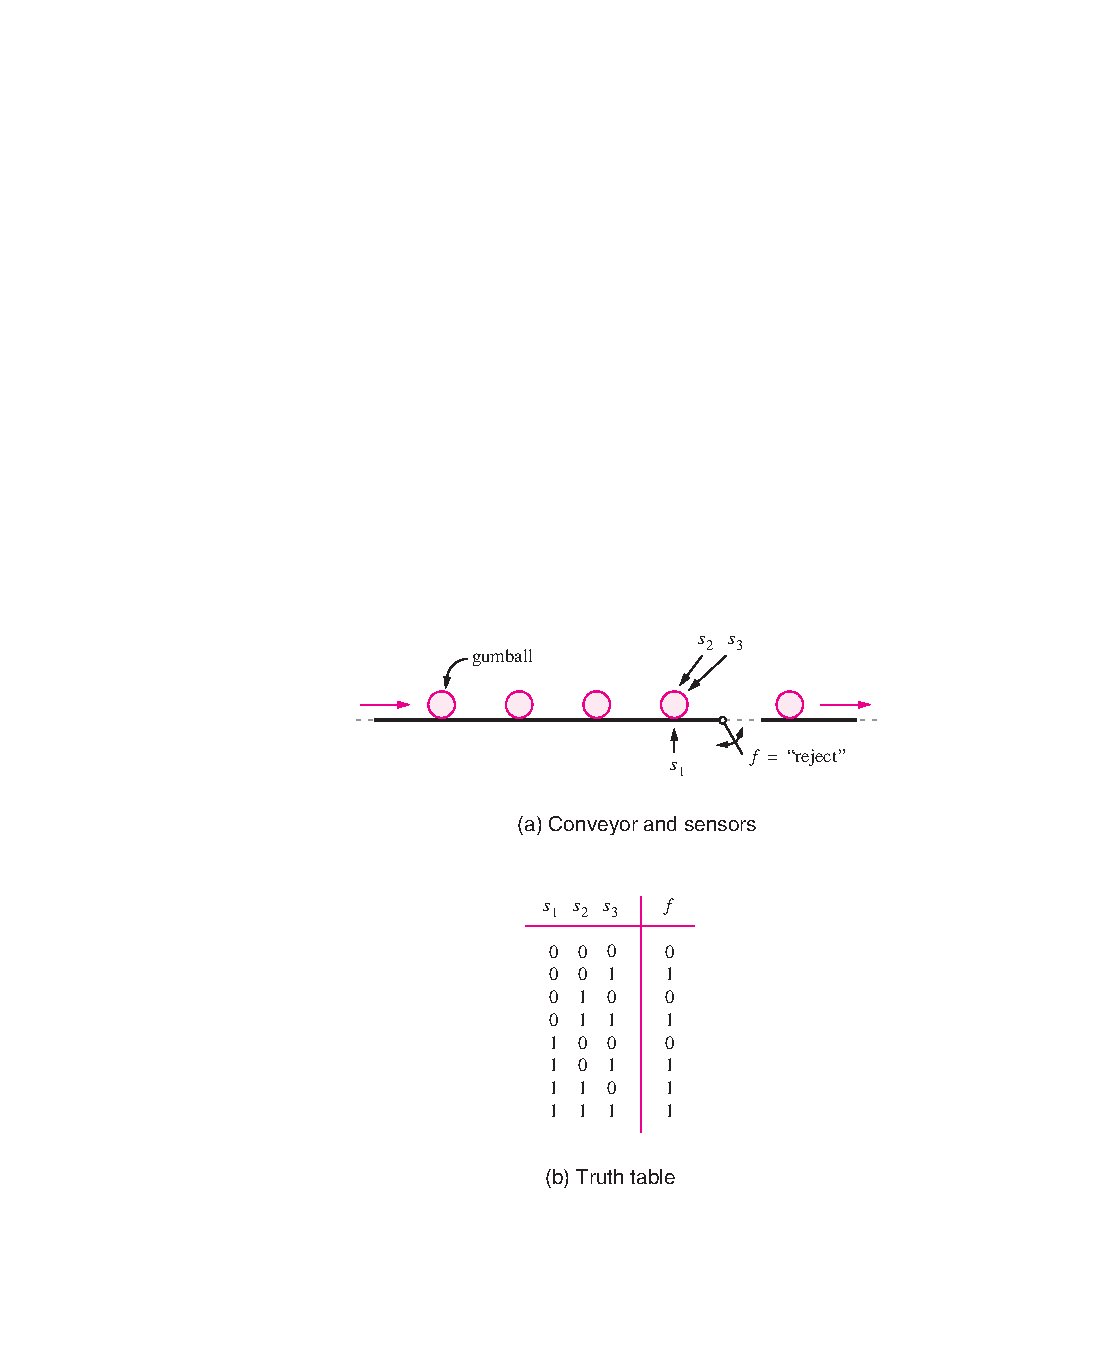
\includegraphics[width=\textwidth]{VerilogFig2_21}
            \vspace{1cm}            \tiny
            $f(s_1,s_2,s_3)=
            \overline{s}_1\overline{s}_2s_3+\overline{s}_1s_2s_3+s_1\overline{s}_2s_3+s_1s_2\overline{s}_3+s_1s_2s_3$
        \end{column}        
        \begin{column}{0.55\textwidth}
            \tiny
            $\overline{s}_1\overline{s}_2s_3+\overline{s}_1s_2s_3+s_1\overline{s}_2s_3+s_1s_2s_3+s_1s_2\overline{s}_3+s_1s_2s_3$ \\
            $\overline{s}_1s_3(\overline{s}_2+s_2)+s_1s_3(\overline{s}_2+s_2)+s_1s_2(\overline{s}_3+s_3)$ \\
            $\overline{s}_1s_3+s_1s_3+s_1s_2$ \\
            $s_3+s_1s_2$ \\
            \vspace{0.3cm}
            ou \\
            \vspace{0.3cm}
            $\overline{s}_1\overline{s}_2s_3+\overline{s}_1s_2s_3+s_1\overline{s}_2s_3+s_1s_2s_3+s_1s_2\overline{s}_3+s_1s_2s_3$ \\
            $s_3(\overline{s}_1\overline{s}_2+\overline{s}_1s_2+s_1\overline{s}_2+s_1s_2)+s_1s_2(\overline{s}_3+s_3)$ \\
            $s_3.1+s_1s_2$ \\
            $s_3+s_1s_2$ \\
            \vspace{0.3cm}
            ou \\
            \vspace{0.3cm}
            $\overline{s}_1\overline{s}_2s_3+\overline{s}_1s_2s_3+s_1\overline{s}_2s_3+\overline{s}_1\overline{s}_2s_3+s_1s_2\overline{s}_3+s_1s_2s_3$ \\
            $\overline{s}_1s_3(s_2+\overline{s}_2)+\overline{s}_2s_3(s_1+\overline{s}_1)+s_1s_2(s_3+\overline{s}_3)$ \\
            $\overline{s}_1s_3+\overline{s}_2s_3+s_1s_2$ \\
            $s_3(\overline{s}_1+\overline{s}_2)+s_1s_2$ \\
            $s_3(\overline{s_1s_2})+s_1s_2$ \\
            $s_3+s_1s_2$ \\
        \end{column}
    \end{columns}
}

\frame{
    \centering
    \frametitle{Mintermos e maxtermos}
    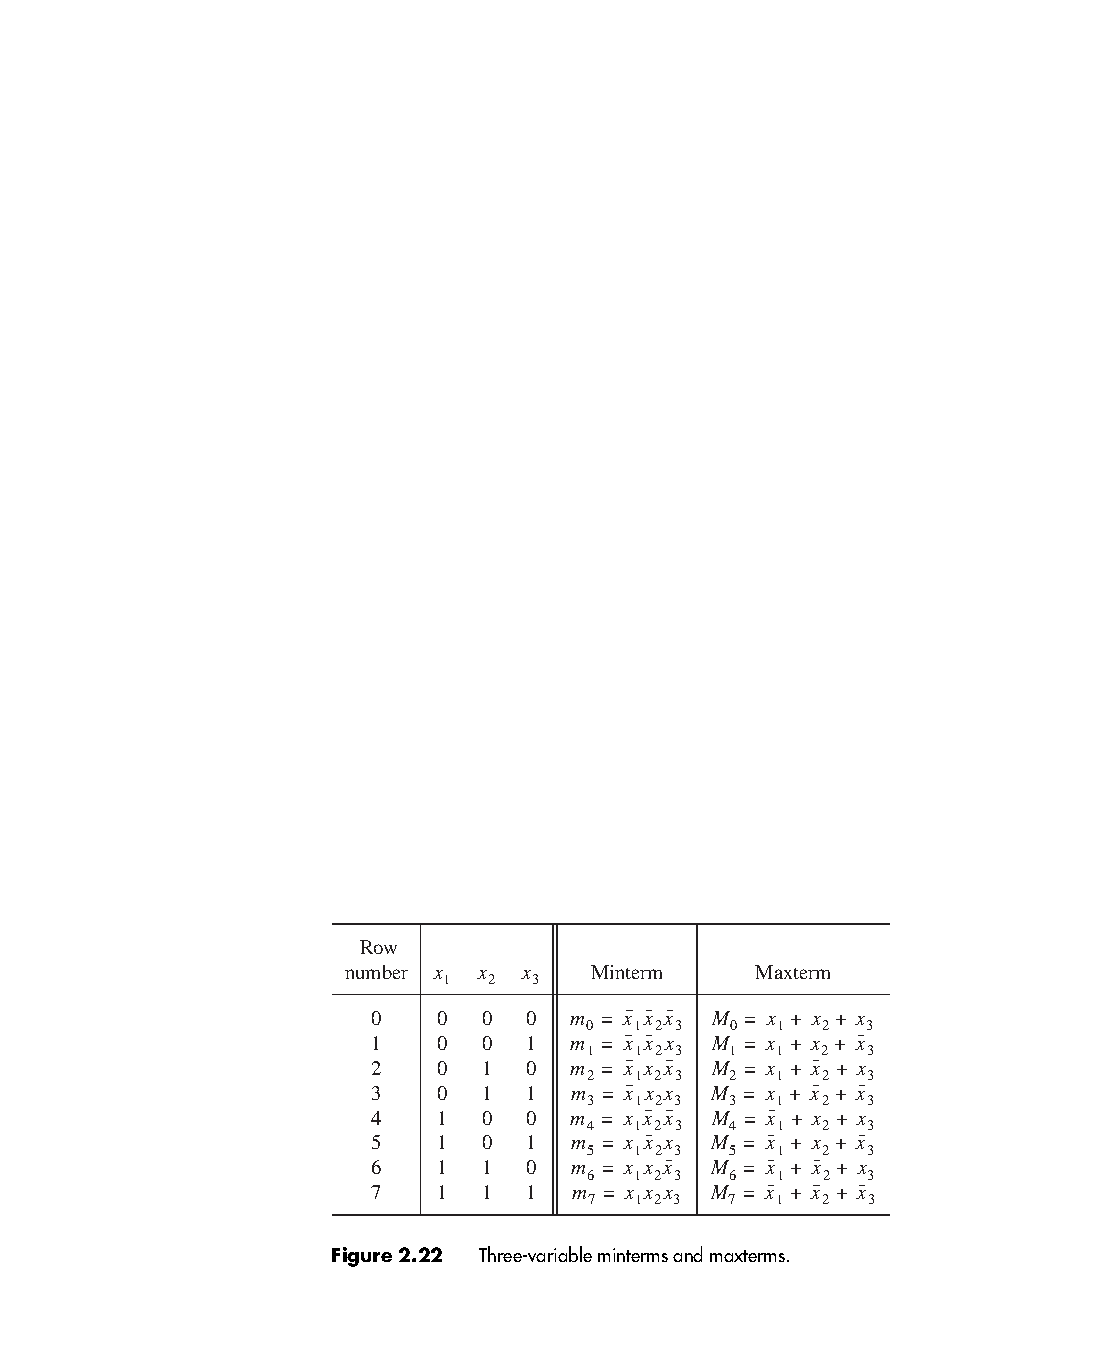
\includegraphics{VerilogFig2_22} \\
}
%NOTE: A good indication of the cost of a logic circuit is the total number of gates plus the total number of inputs to all gates in the circuit. Using this measure, the cost of the network in Figure 2.19a is 13, because there are five gates and eight inputs to the gates.

\frame{     \centering
    \frametitle{Formas canônicas}
    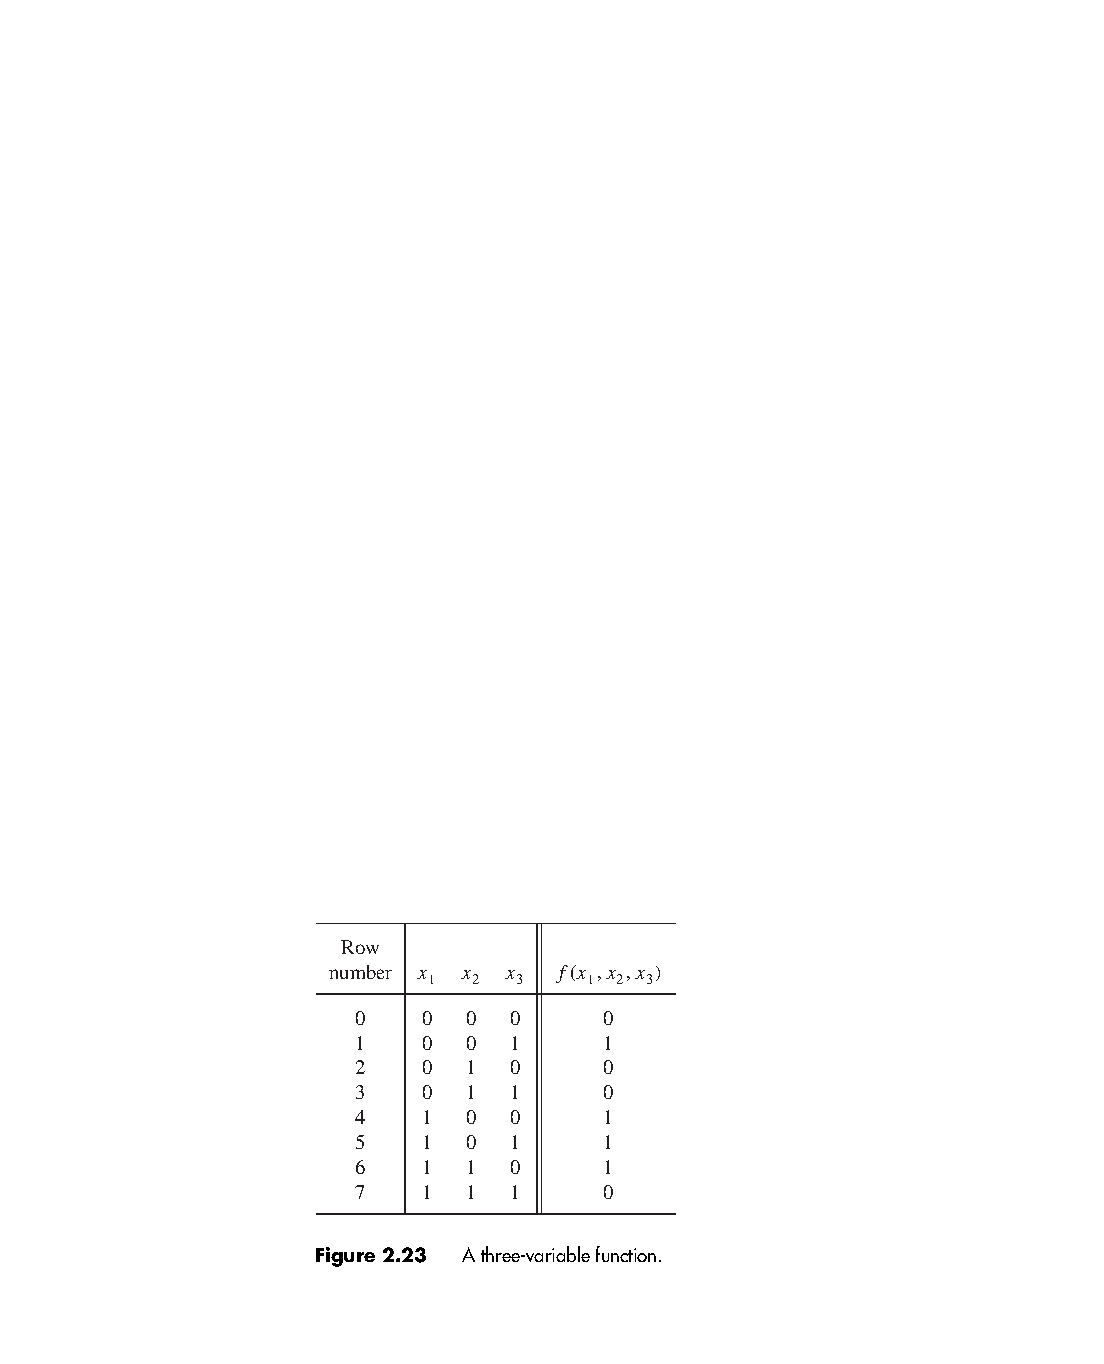
\includegraphics[scale=.9]{VerilogFig2_23} \\
    \vspace{0.5cm}
    \small
    \begin{tabular}{cc}
        Soma dos produtos: & Produto das somas: \\
        $f(x_1, x_2, x_3) = \Sigma (m_1, m_4, m_5, m_6)$ & $f(x_1, x_2, x_3) = \Pi (M_0, M_2, M_3, M_7)$ \\    
        $f(x_1, x_2, x_3) = \Sigma m(1, 4, 5, 6)$ & $f(x_1, x_2, x_3) = \Pi M(0, 2, 3, 7)$ \\
    \end{tabular}
}

\frame{     \centering
    \frametitle{Formas canônicas}
    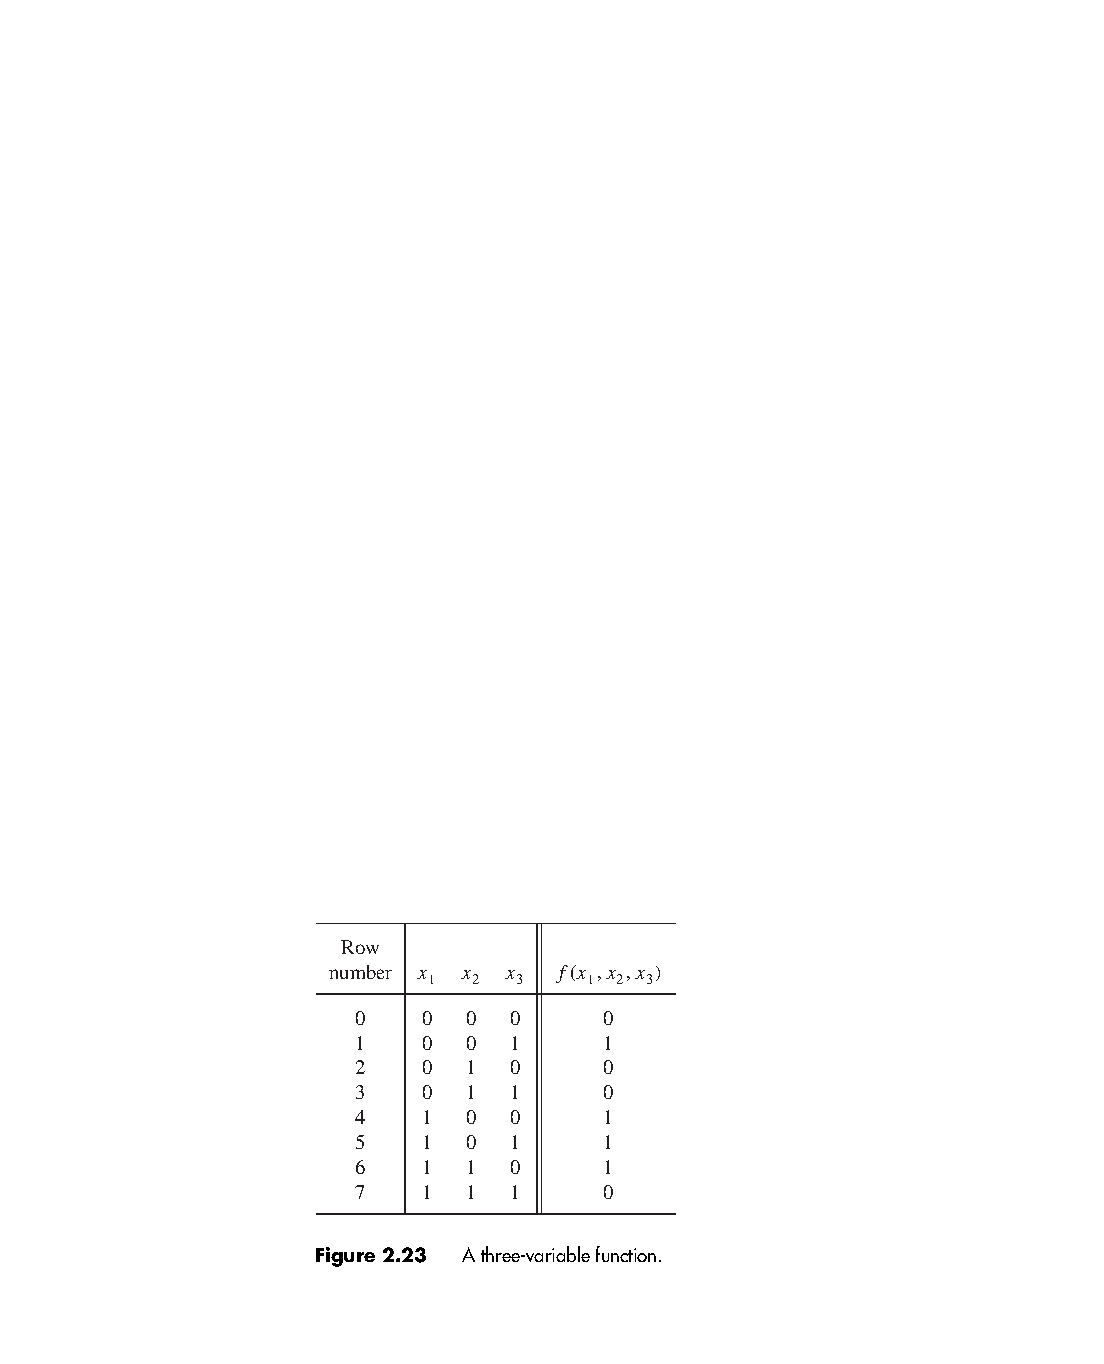
\includegraphics[scale=.8]{VerilogFig2_23} \\
    \vspace{0.5cm}
    \small
    $\overline{f}=m_0+m_2+m_3+m_7$ \\
    $f=\overline{m_0+m_2+m_3+m_7}$ \\
    $f=\overline{m}_0\overline{m}_2\overline{m}_3\overline{m}_7$ \\
    $f=M_0.M_2.M_3.M_7$ \\
}

\frame{     \centering
    \frametitle{Implementações possíveis para a função}
    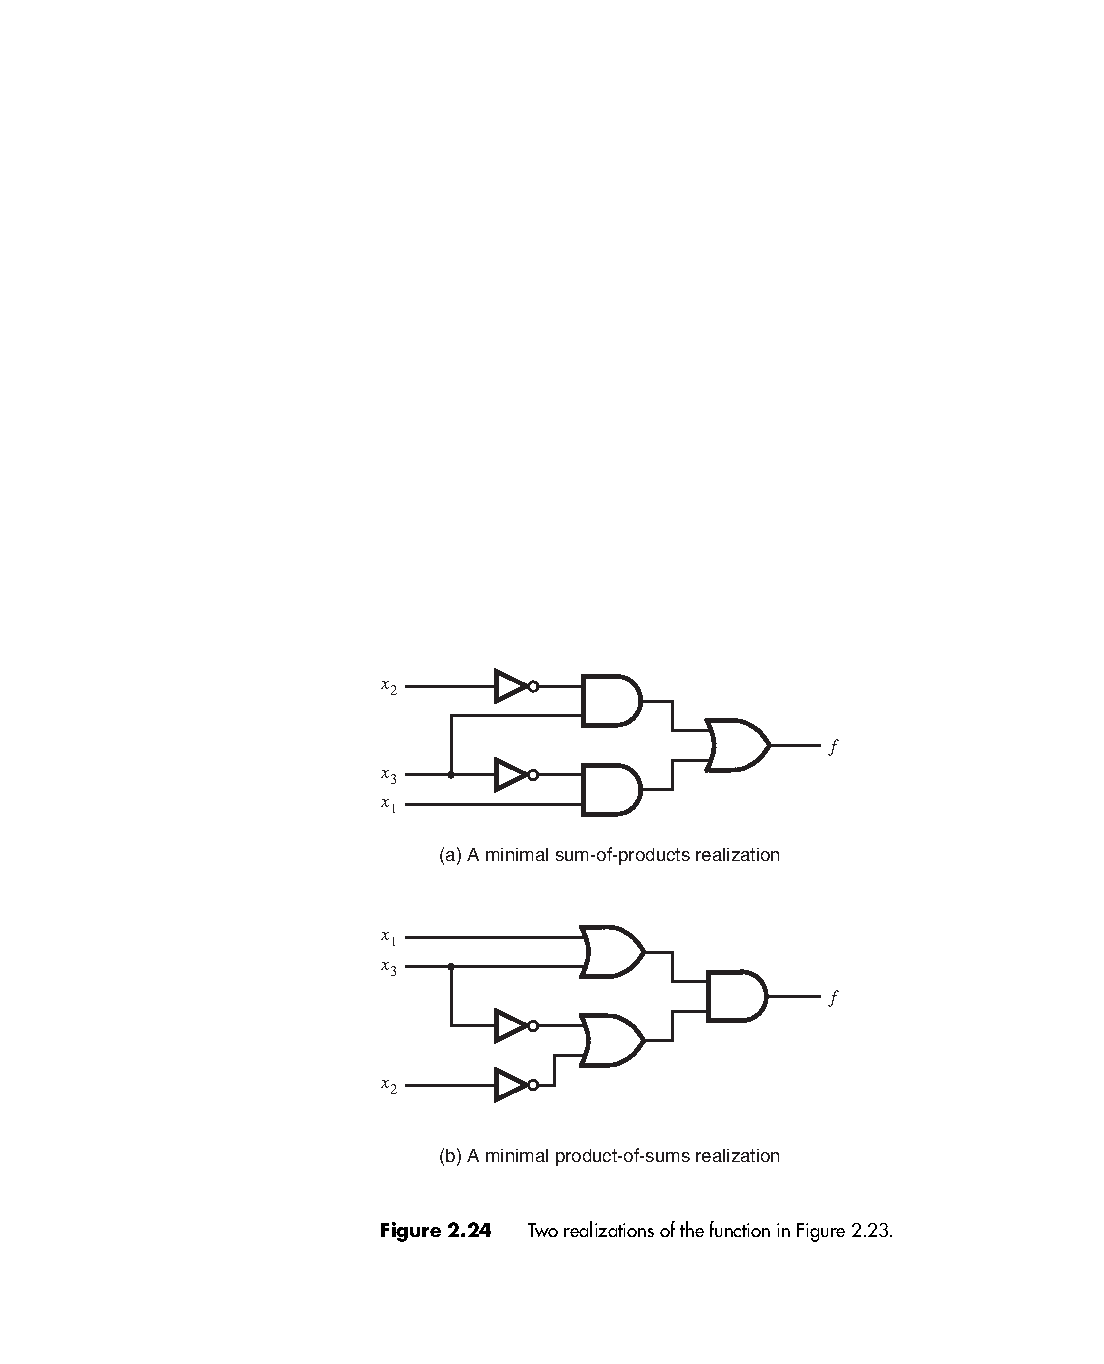
\includegraphics[scale=.8]{VerilogFig2_24}
}

\frame{     \centering
    \frametitle{Portas NAND e NOR}
    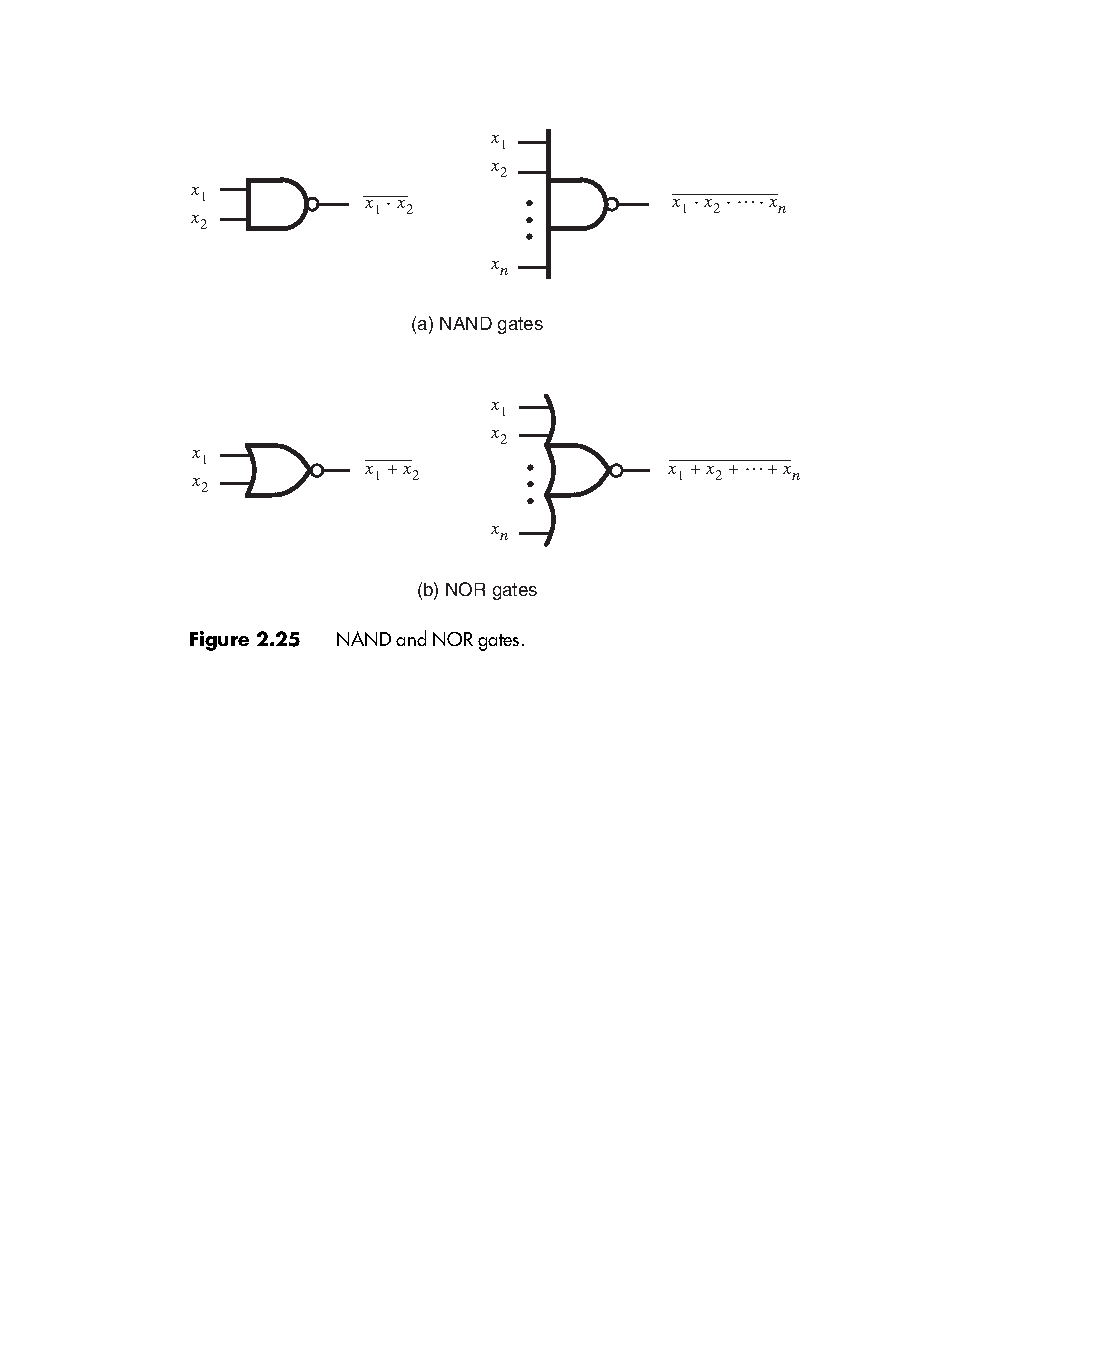
\includegraphics[scale=.8]{VerilogFig2_25}
}

\frame{     \centering
    \frametitle{Teorema DeMorgan}
    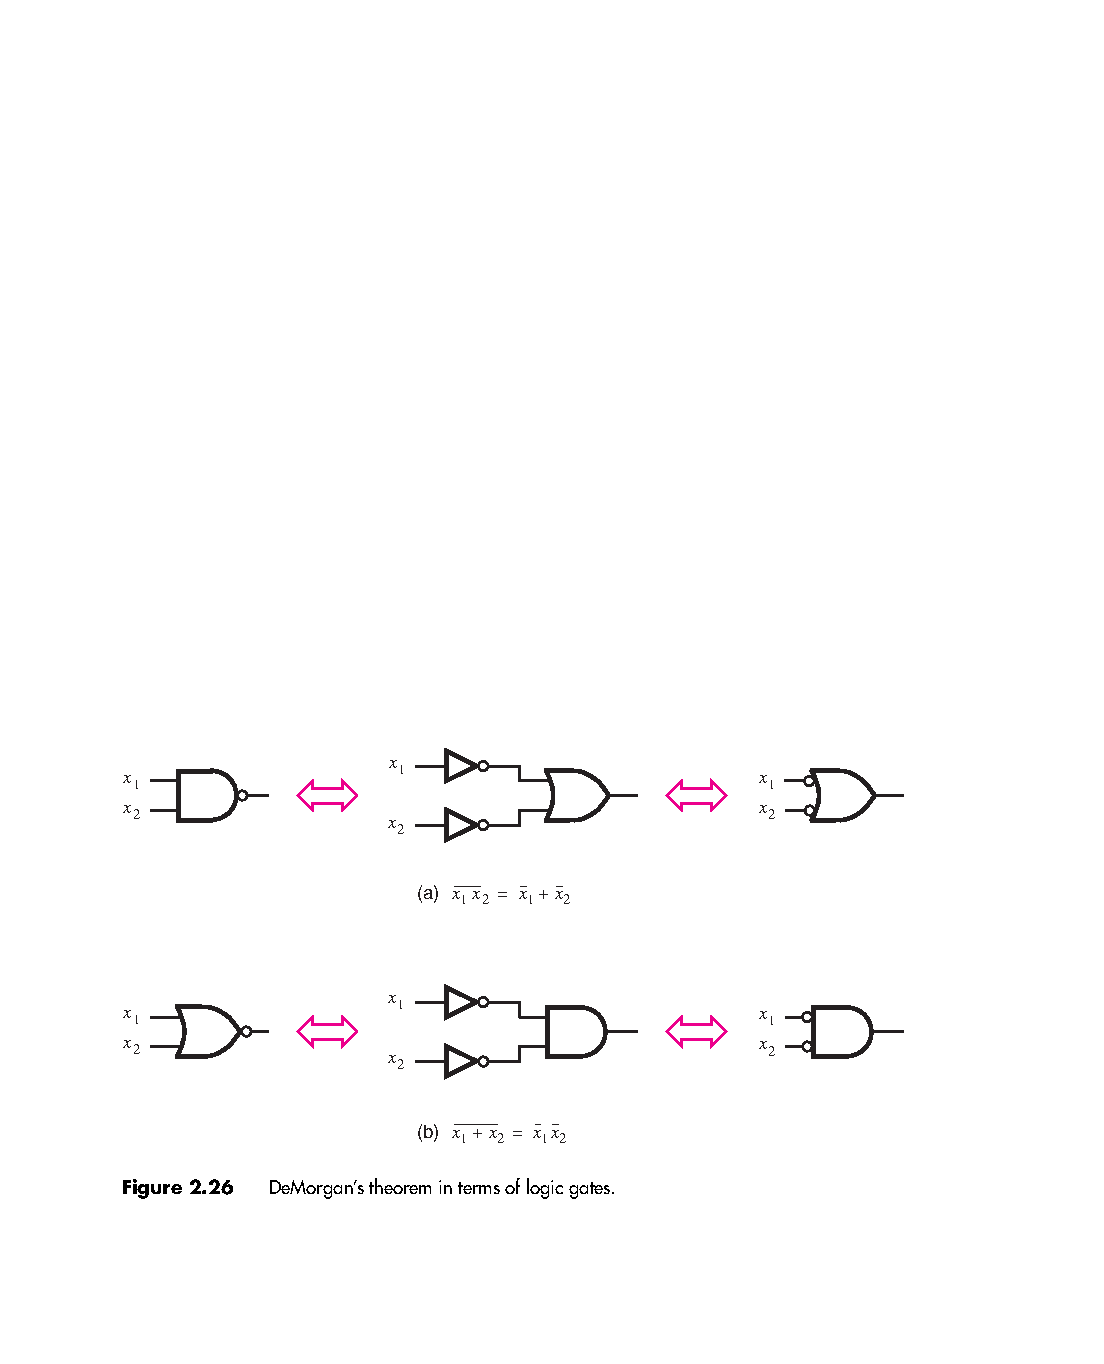
\includegraphics[scale=.9]{VerilogFig2_26}
}

\section{Exemplos}

\frame{     \centering
    \frametitle{\insertsection}
    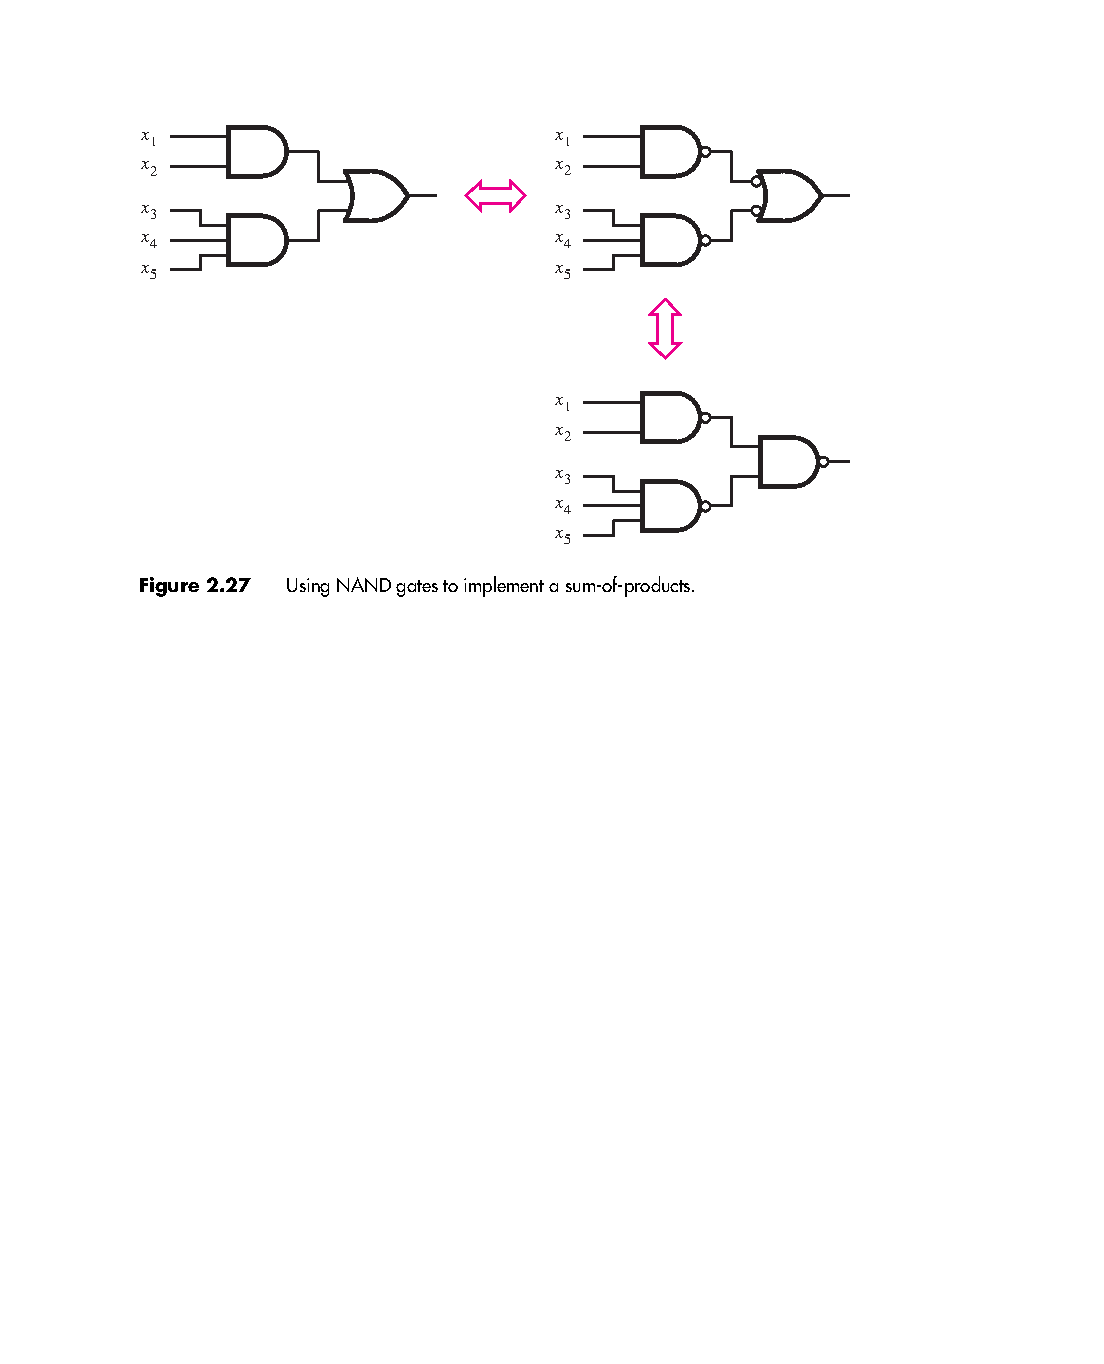
\includegraphics[scale=.8]{VerilogFig2_27}
}

\frame{     \centering
    \frametitle{\insertsection}
    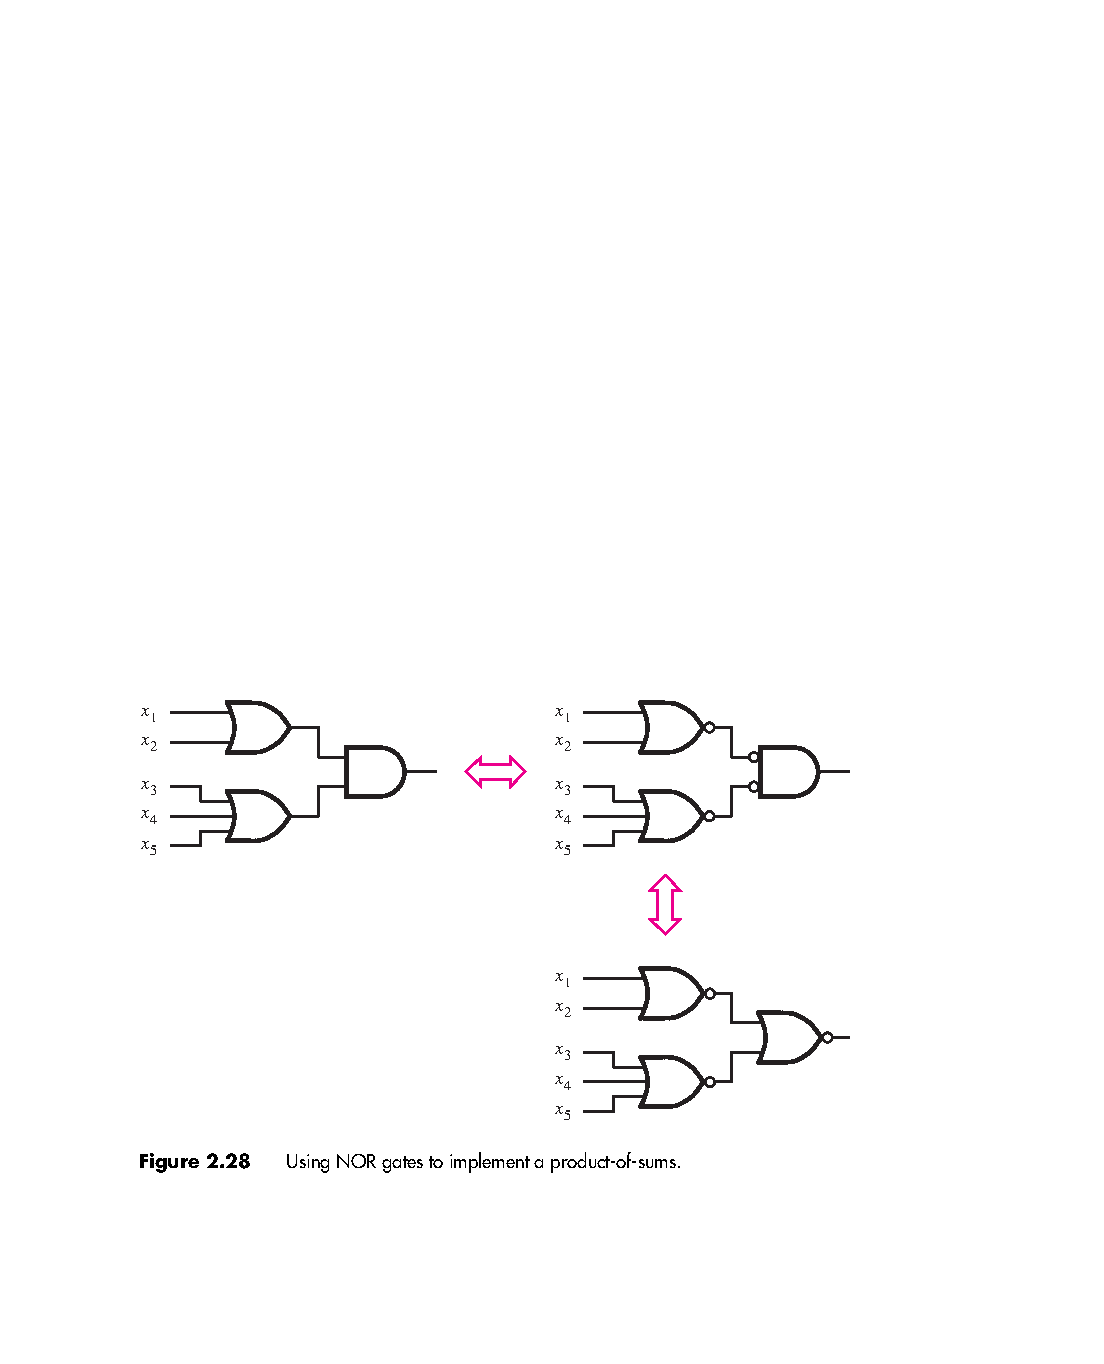
\includegraphics[scale=.8]{VerilogFig2_28}
}

\frame{     \centering
    \frametitle{\insertsection}
    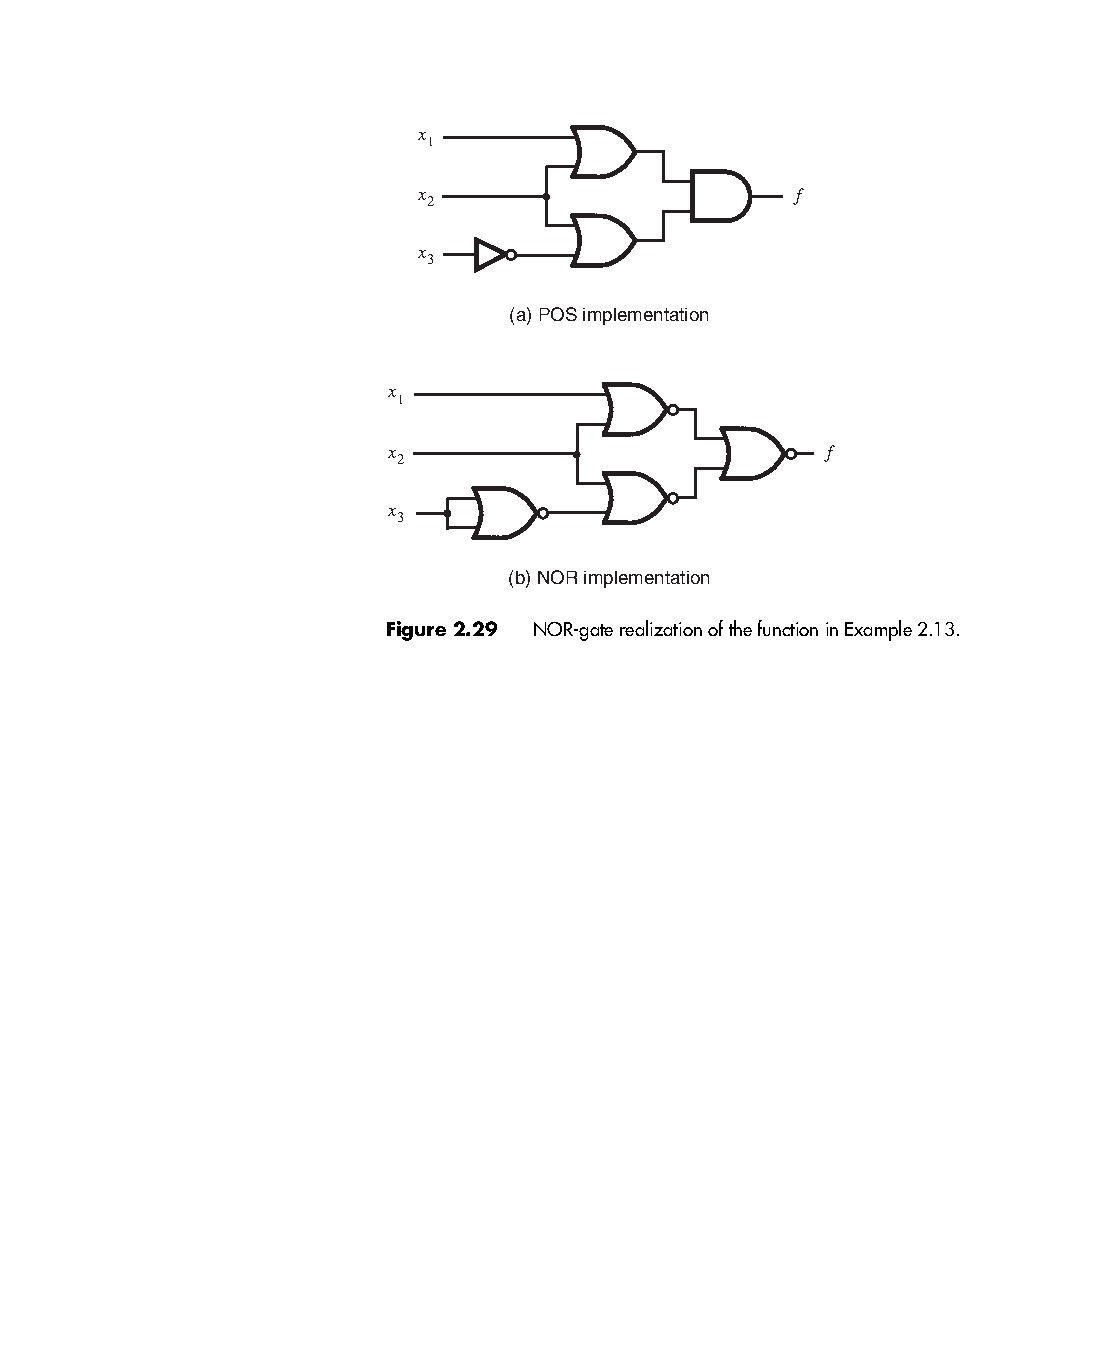
\includegraphics[scale=.8]{VerilogFig2_29}
}

\frame{     \centering
    \frametitle{\insertsection}
    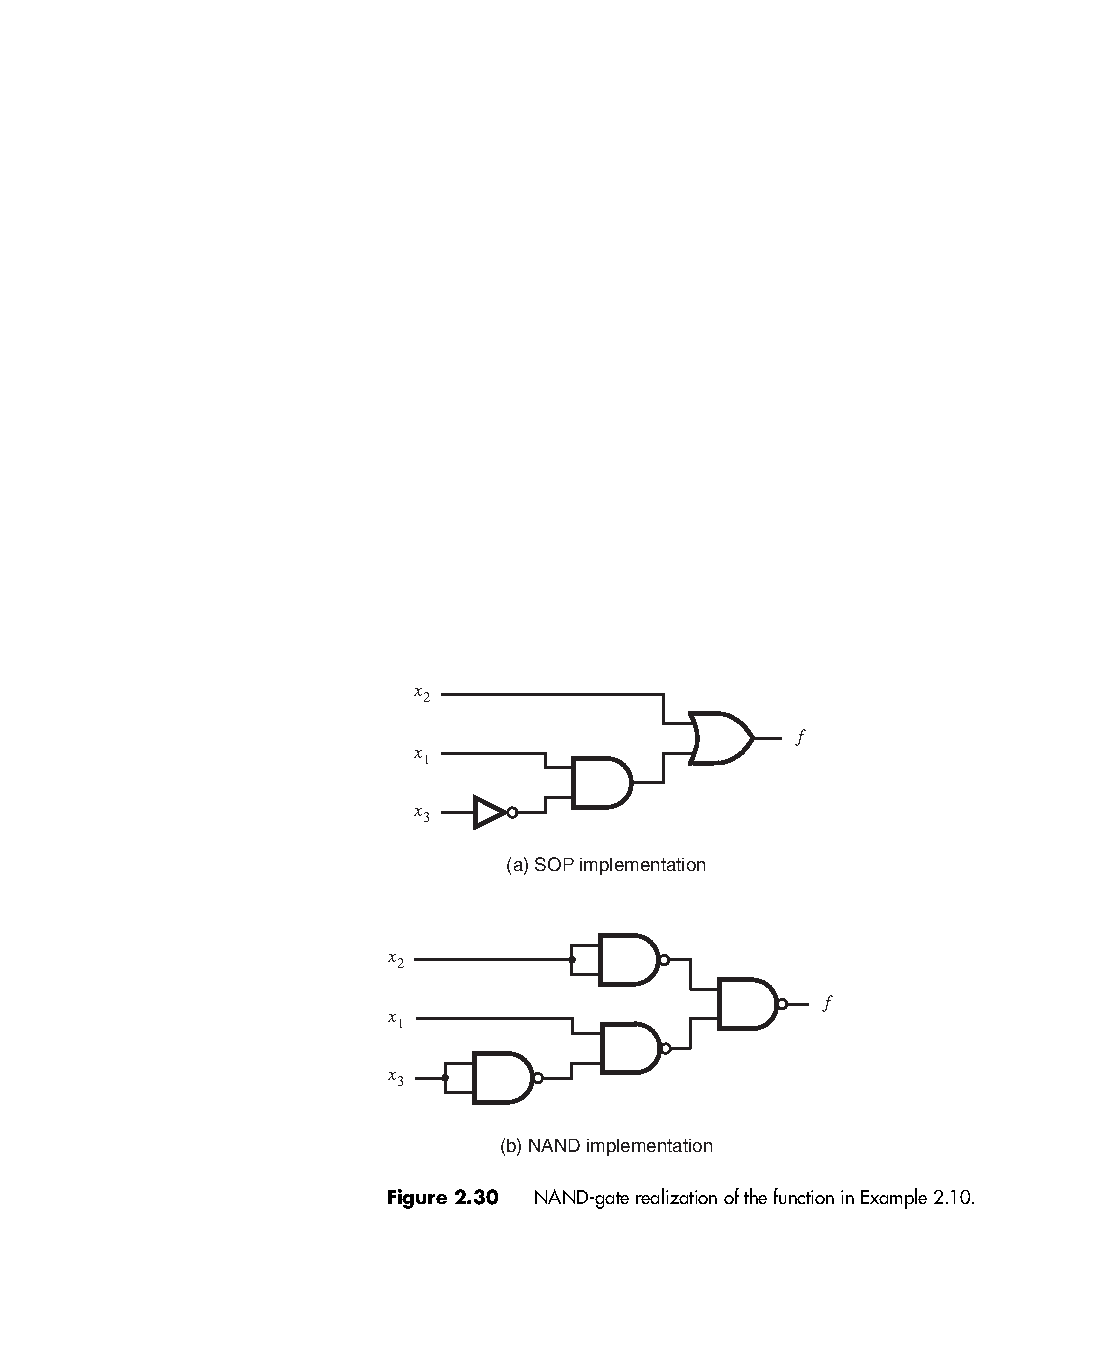
\includegraphics[scale=.8]{VerilogFig2_30}
}





\section{Bibliografia} %%%%%%%

\begin{frame}{\insertsection} 
	\begin{itemize}
		\item \href{https://www.google.com.br/search?q=filetype\%3Apdf+Fundamentals+of+Digital+Logic+with+Verilog+Design+&oq=filetype\%3Apdf}{Brown, S. \& Vranesic, Z. - Fundamentals of Digital Logic with Verilog Design, 3rd Ed., Mc Graw Hill, 2009}
	\end{itemize}
\end{frame}

\begin{frame}
	\titlepage
\end{frame} 

\end{document}